\documentclass{article}
\usepackage{graphicx}
\usepackage{hyperref}
\usepackage{tikz}
\usetikzlibrary{positioning}

\title{[Draft] RISE pevm: Blazingly Fast Parallel Executor for EVM Blockchains}
\author{Hai Nguyen \\ hai@riselabs.xyz}
\date{September 2024}

\begin{document}

\maketitle

\begin{abstract}

    RISE pevm is a parallel EVM executor heavily inspired by Block-STM. We made several contributions to improve
    performance, especially when Aptos designed Block-STM for MoveVM instead of EVM. Most notable is the introduction
    of lazy updates to remove explicit reads and dependencies in common transaction scenarios. Our implementation is
    open-source at \url{https://github.com/risechain/pevm}. The reproducible benchmarks show that RISE pevm is the
    fastest EVM block executor, with a peak speedup of 22x and a peak raw execution throughput of 55 Gigagas/s on 32
    AWS Graviton3 CPUs. RISE pevm also enables new possibilities for parallel EVM dApp designs.

\end{abstract}

\section{Introduction}

Parallelizing execution to accelerate blockchain throughput has gained popularity thanks to Aptos, Sui, and Solana.
However, it is still unfruitful in the EVM land. Early adaptions of Block-STM\cite{blockstm} by Polygon and Sei have
shown limited speedup due to the lack of EVM-specific optimizations and implementation limitations. Both Polygon and
Sei use Go, a garbage-collected language unsuitable for optimizations at the micro-second scale. Parallel execution in
Go is mostly slower than sequential execution in Rust and C++ for Ethereum mainnet blocks today.

RISE pevm sets to address this problem by designing an EVM-specialized parallel executor and implementing it in
Rust to minimize runtime overheads. The result is the fastest EVM block executor, with a peak speedup of 22x and a
raw execution throughput of 55 Gigagas/s on 32 AWS Graviton3 CPUs. RISE pevm also enables new parallel dApp designs for
EVM like Sharded AMM\cite{samm}.

While others embed their parallel executor directly into their nodes, we built a dedicated repository to
serve as a playground for further pevm R\&D. The code base is open-source at \url{https://github.com/risechain/pevm}.

\section{Foundation}

Blockchain execution must be deterministic for network participants to agree on blocks and state transitions.
Therefore, parallel execution must arrive at the same outcome as sequential execution. Having race conditions that
affect execution results would break consensus.

\subsection{Block-STM}

RISE pevm builds on Block-STM's optimistic execution based on Software Transaction Memory\cite{stm} and Optimistic
Concurrency Control\cite{occ}. We also use a multi-version data structure to record the memory locations that each
transaction reads and writes to. The collaborative scheduler has validation tasks to re-execute transactions that
yielded state conflicts. The scheduler finishes when all transactions pass validation and arrives at the same result
with sequential execution.

\section{Contributions}

We made several contributions both generally and fine-tuned for EVM.

\subsection{Lazy Updates}

All EVM transactions in the same block read and write to the beneficiary account for gas payment, making all
transactions interdependent by default. RISE pevm addresses this by lazy-updating the beneficiary balance. We mock the
balance on gas payment reads to avoid registering a state dependency and only evaluate it at the end of the block or
when there is an explicit read. We apply the same technique for common scenarios like raw ETH and ERC-20 transfers.
Lazy updates help us parallelize transfers from and to the same address, with only a minor post-processing latency for
evaluating the lazy values.

\section{Architecture}

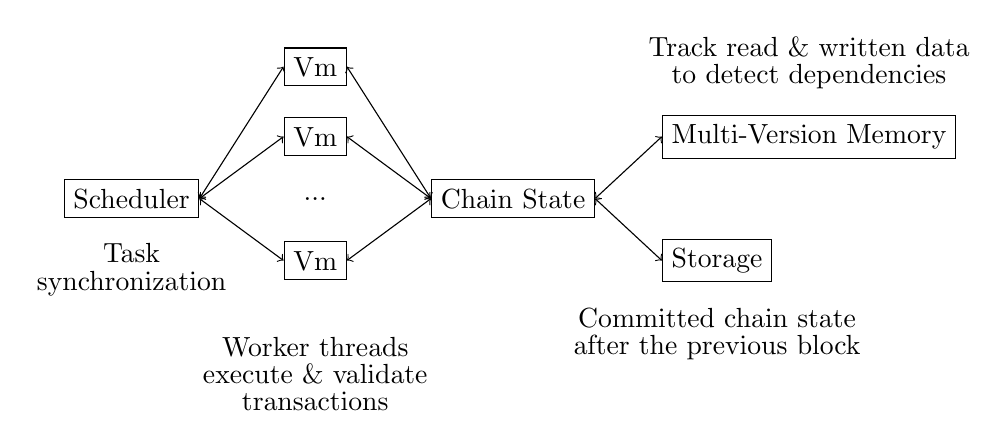
\begin{tikzpicture}[rect/.style={rectangle, draw=black}]
    % Nodes
    \node[rect] (scheduler) {Scheduler};
    \node [below=0.2cm of scheduler] {\shortstack{Task\\synchronization}};

    \node (morevm) [right=1.2cm of scheduler] {...};
    \node[rect] (vm2) [above=0.4cm of morevm] {Vm};
    \node[rect] (vm1) [above=0.4cm of vm2] {Vm};
    \node[rect] (vm3) [below=0.4cm of morevm] {Vm};
    \node [below=0.6cm of vm3] {\shortstack{Worker threads\\execute \& validate\\transactions}};

    \node[rect] (state) [right=1.2cm of morevm] {Chain State};

    \node[rect] (mv) [right=4cm of vm2] {Multi-Version Memory};
    \node [above=0.2cm of mv] {\shortstack{Track read \& written data\\to detect dependencies}};
    \node[rect] (storage) [right=4cm of vm3] {Storage};
    \node [below=0.2cm of storage] {\shortstack{Committed chain state\\after the previous block}};

    % Arrows
    \draw[<->] (scheduler.east) -- (vm1.west);
    \draw[<->] (scheduler.east) -- (vm2.west);
    \draw[<->] (scheduler.east) -- (vm3.west);

    \draw[<->] (vm1.east) -- (state.west);
    \draw[<->] (vm2.east) -- (state.west);
    \draw[<->] (vm3.east) -- (state.west);

    \draw[<->] (state.east) -- (mv.west);
    \draw[<->] (state.east) -- (storage.west);
\end{tikzpicture}

\section{Implementation}

\section{Integration}

\section{Evaluation}

\section{Future Works}

\subsection{Preprocessed Dependencies}

We can add a list of preprocessed dependencies to the scheduler to only execute a transaction after executing all of
its dependencies. This list can be computed internally by pevm inspecting the input block or externally by an advanced
mempool. While this technique helps minimize re-execution, it still resorts to sequential execution for dependent
transactions. Lazy updates are much more potent as they execute dependent transactions in parallel for only a minor
post-processing cost. For instance, we used to pre-define dependencies across transactions of the same sender and
recipient, which we eventually replaced with lazy updates for 2-3x speedup. Nevertheless, this technique remains
helpful for state dependencies that cannot yet be lazy-updated.

\subsection{Extended Block Metadata}

Block builders and executors can inspect each transaction's final read and write set for valuable metadata that
improves downstream execution speed.

\textbf{Transaction Dependency Graph}: Syncing nodes can fork-join block execution according to a transaction
dependency graph. Each parallel fork executes a chain of dependent transactions sequentially. All forks join at the end
for post-processing. This optimal process yields no state conflict and re-execution. A single full-block validation at
the end confirms the execution result.

\textbf{Read Memory Locations}: Syncing nodes can concurrently preload to-be-read memory locations to avoid blocking
I/O during transaction execution.

\textbf{Blacklisting}: Malicious metadata like enormous read memory locations can significantly slow down or even crash
syncing nodes. Therefore, syncing nodes must have strict bounds while parsing and blacklist nodes that provide bad
metadata, either to not receive more blocks or to not process extended metadata from them. Sensitive nodes can go
further by only whitelisting trusted nodes. Nevertheless, if the full-block validation fails after executing with a
dependency graph, the syncing node can still fall back to optimistic execution.

\section{Conclusion}

\begin{thebibliography}{1}

    \bibitem{blockstm} Rati Gelashvili, Alexander Spiegelman, Zhuolun Xiang, George Danezis, Zekun Li, Dahlia Malkhi,
    Yu~Xia, and Runtian Zhou. Block-stm: Scaling blockchain execution by turning ordering curse to a performance
    blessing (2022).

    \bibitem{samm} Hongyin Chen and Amit Vaisman and Ittay Eyal. SAMM: Sharded Automated Market Maker (2024).

    \bibitem{stm} Nir Shavit and Dan Touitou. 1997. Software transactional memory. Distributed Computing 10, 2 (1997),
    99–116.

    \bibitem{occ} H. T. Kung and John T. Robinson. 1981. On optimistic methods for concurrency control. ACM Trans.
    Database Syst. 6, 2 (June 1981), 213–226.

\end{thebibliography}

\end{document}
